% Ready-to-insert result figures and tables generated from the inclusive archive.
% Place each block at the location documented in PAPER_FIGURE_PLAN.md.

% --- Overall Accuracy and Conditional Doubt Effect ---
\begin{figure*}[t]
  \centering
  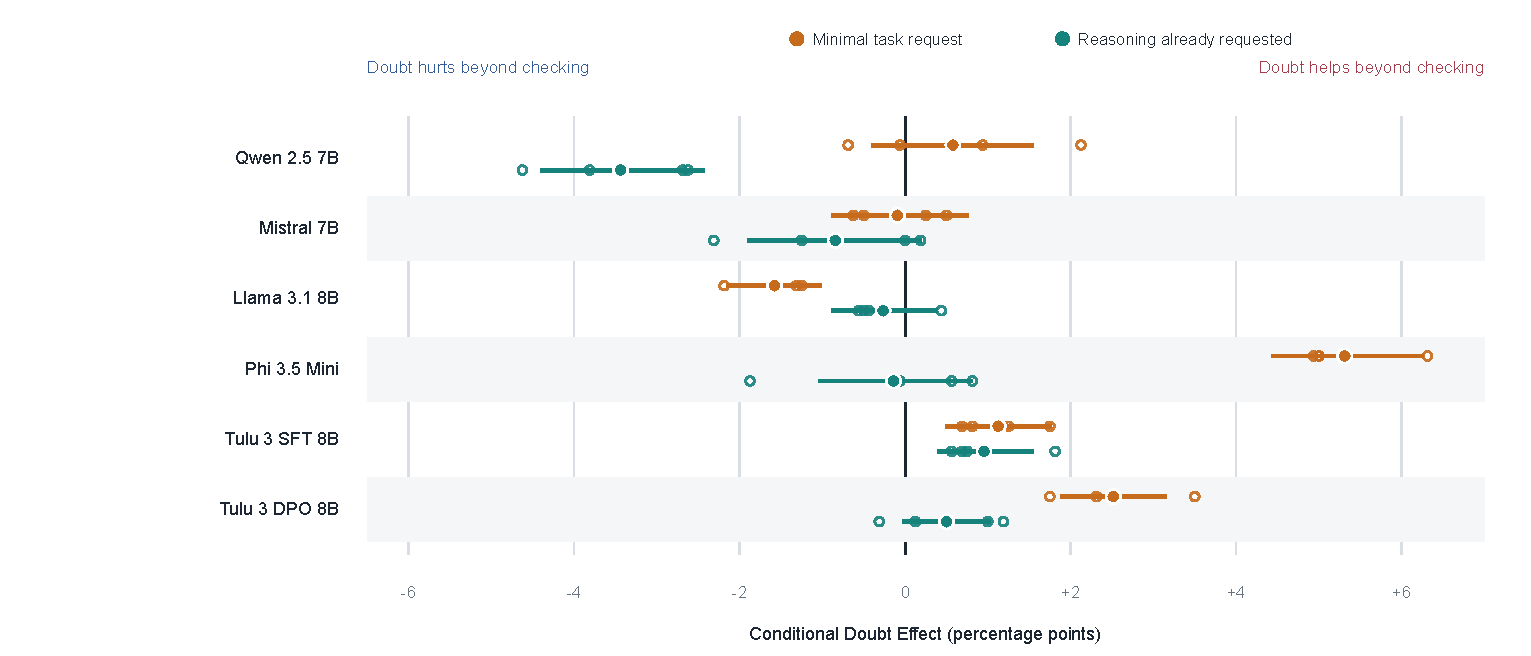
\includegraphics[width=.94\textwidth]{figures/results/cde_context_forest.pdf}
  \caption{Conditional Doubt Effect (CDE) by checkpoint and task context. Open
  circles show the four independent task seeds, filled circles show the
  seed--family macro mean, and horizontal lines are paired 95\% task-bootstrap
  intervals. Adding self-doubt after checking is not uniformly beneficial: its
  sign and magnitude depend on both checkpoint and whether the task already
  requests reasoning.}
  \label{fig:cde-context}
\end{figure*}

\begin{table*}[t]
\centering
\caption{Inclusive \bench{} scorecard over all structurally complete cells.
Neutral is an accuracy percentage; all other entries are percentage-point
effects. CDE intervals are paired task-bootstrap intervals conditional on the
four frozen task seeds. Tulu checkpoints share a Llama-3.1 foundation lineage.}
\label{tab:main-results}
\scriptsize
\begin{tabular}{@{}lrrrrrrr@{}}
\toprule
\textbf{Checkpoint} & $A_N$ & $A_C-A_N$ & \textbf{CDE [95\% CI]} & CDE$_{\min}$ & CDE$_{\mathrm{reason}}$ & \textbf{CM} & $A_{C+Q}-A_C$ \\
\midrule
Qwen 2.5 7B   & 66.44 & +7.70 & $-1.43\;[-2.14,-0.69]$ & +0.58 & -3.44 & -4.02 & -27.05 \\
Mistral 7B    & 24.96 & +0.51 & $-0.47\;[-1.14,+0.20]$ & -0.09 & -0.84 & -0.75 & +1.10 \\
Llama 3.1 8B & 20.00 & +1.45 & $-0.92\;[-1.34,-0.49]$ & -1.58 & -0.27 & +1.31 & -5.63 \\
Phi 3.5 Mini  & 44.98 & +0.45 & $+2.59\;[+1.95,+3.27]$ & +5.31 & -0.14 & -5.45 & -7.53 \\
Tulu 3 SFT 8B & 13.52 & -0.12 & $+1.04\;[+0.60,+1.48]$ & +1.13 & +0.95 & -0.17 & +1.32 \\
Tulu 3 DPO 8B & 16.30 & +1.79 & $+1.51\;[+1.12,+1.92]$ & +2.52 & +0.50 & -2.02 & -3.74 \\
\bottomrule
\end{tabular}
\end{table*}

% --- Task-Family and Difficulty Heterogeneity ---
\begin{figure*}[t]
  \centering
  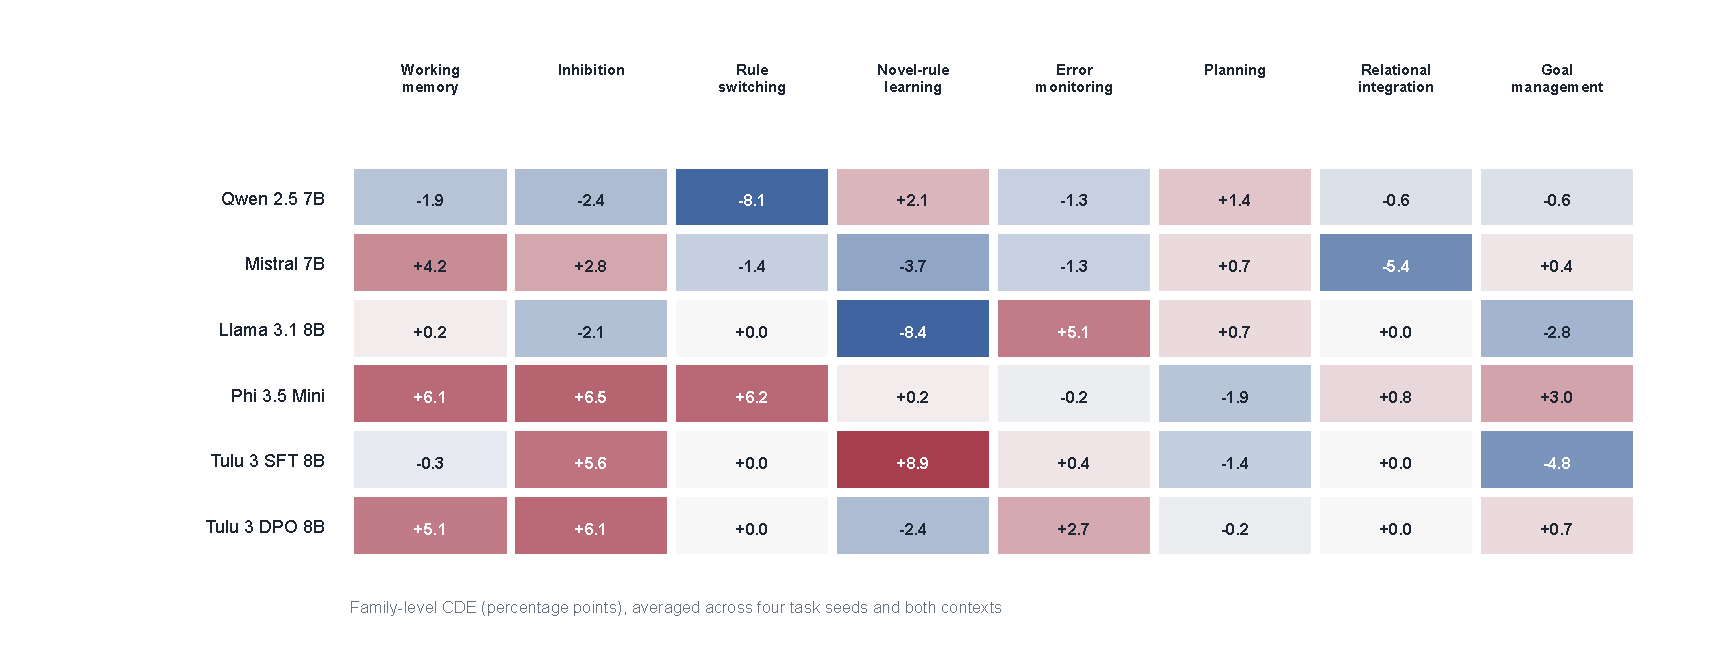
\includegraphics[width=.98\textwidth]{figures/results/family_cde_heatmap.pdf}
  \caption{Task-family CDE in percentage points, averaged across four task
  seeds and both task contexts. Aggregate effects hide structured reversals:
  the same prompt component can help one task family and harm another for the
  same checkpoint. Twenty-one nonzero checkpoint--family directions retain
  their sign in all four task seeds.}
  \label{fig:family-cde}
\end{figure*}

% --- Seed and Surface Robustness ---
\begin{figure*}[t]
  \centering
  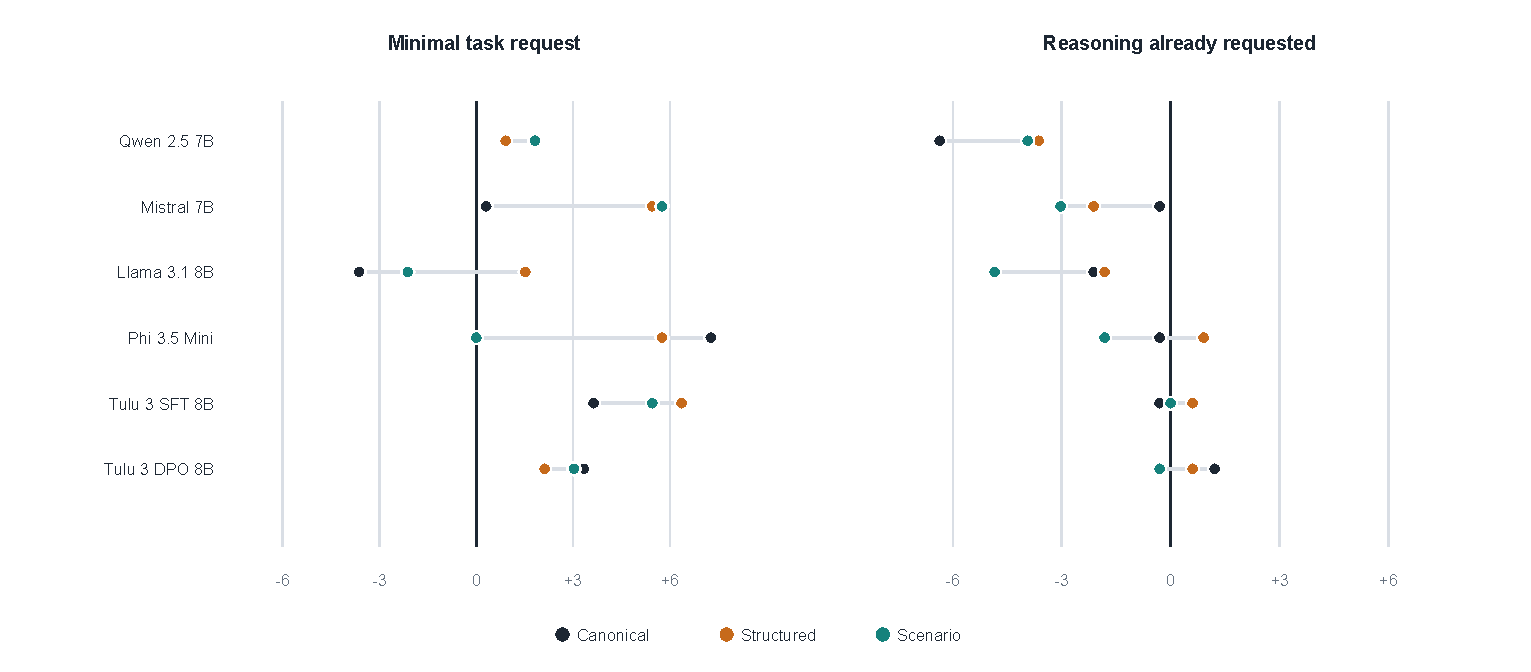
\includegraphics[width=.94\textwidth]{figures/results/surface_cde_robustness.pdf}
  \caption{CDE on 330 held-out latent tasks under canonical, structured, and
  scenario renderings. Mean three-way correctness agreement is 81.3\%, but
  exact effect sizes move with answer-preserving wording and five of 12
  checkpoint--context signs cross zero in at least one rendering.}
  \label{fig:surface-cde}
\end{figure*}

% --- Post-Training Case Study ---
\begin{table}[t]
\centering
\caption{Within-lineage Tulu case study. All entries are percentage points;
$\Delta$ is DPO minus SFT. This is not an independent-family comparison.}
\label{tab:tulu-case}
\small
\begin{tabular}{@{}lrrr@{}}
\toprule
\textbf{Endpoint} & \textbf{SFT} & \textbf{DPO} & $\boldsymbol{\Delta}$ \\
\midrule
Neutral accuracy & 13.52 & 16.30 & +2.78 \\
Checking gain & -0.12 & +1.79 & +1.91 \\
CDE$_{\min}$ & +1.13 & +2.52 & +1.39 \\
CDE$_{\mathrm{reason}}$ & +0.95 & +0.50 & -0.45 \\
CM & -0.17 & -2.02 & -1.84 \\
Concision effect & +1.32 & -3.74 & -5.06 \\
\bottomrule
\end{tabular}
\end{table}

% --- Appendix diagnostics ---
\begin{figure*}[t]
  \centering
  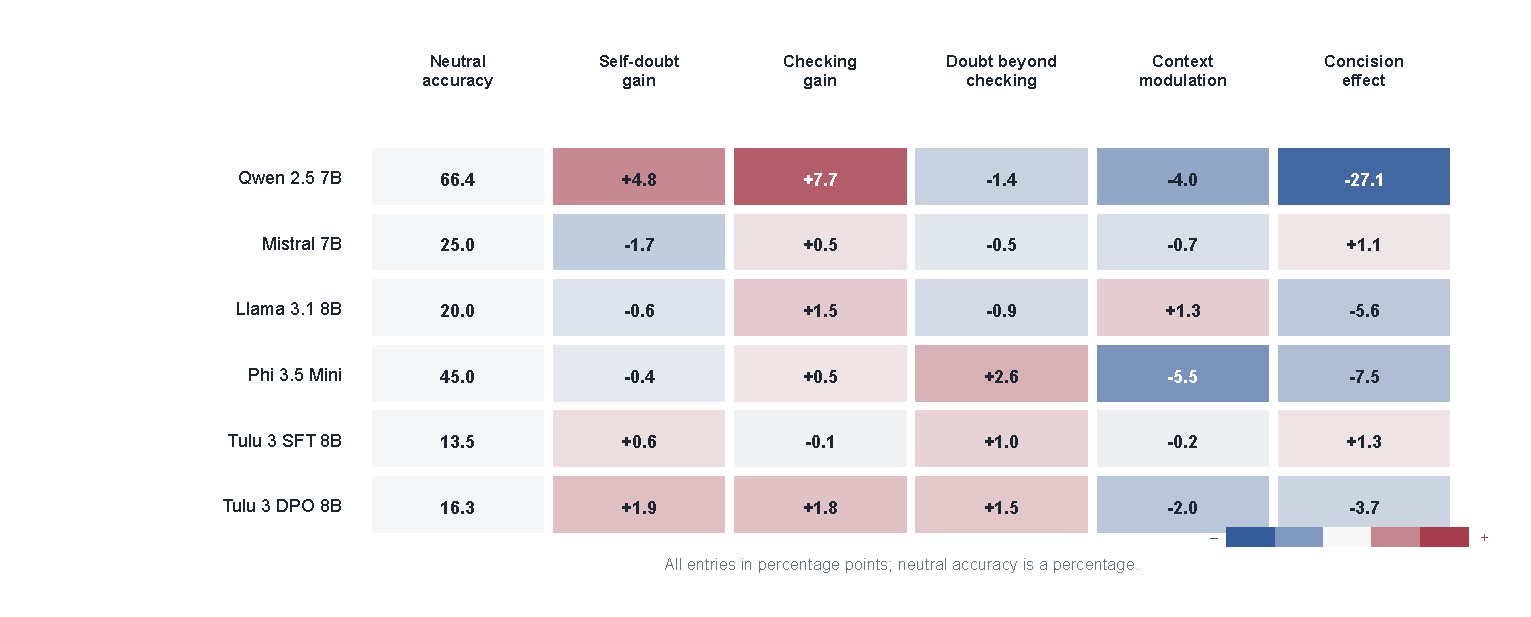
\includegraphics[width=.92\textwidth]{figures/results/inclusive_scorecard_heatmap.pdf}
  \caption{Full inclusive scorecard. Signed cells use a diverging scale; neutral
  accuracy is shown without a signed value judgment.}
  \label{fig:scorecard-heatmap}
\end{figure*}

\begin{figure}[t]
  \centering
  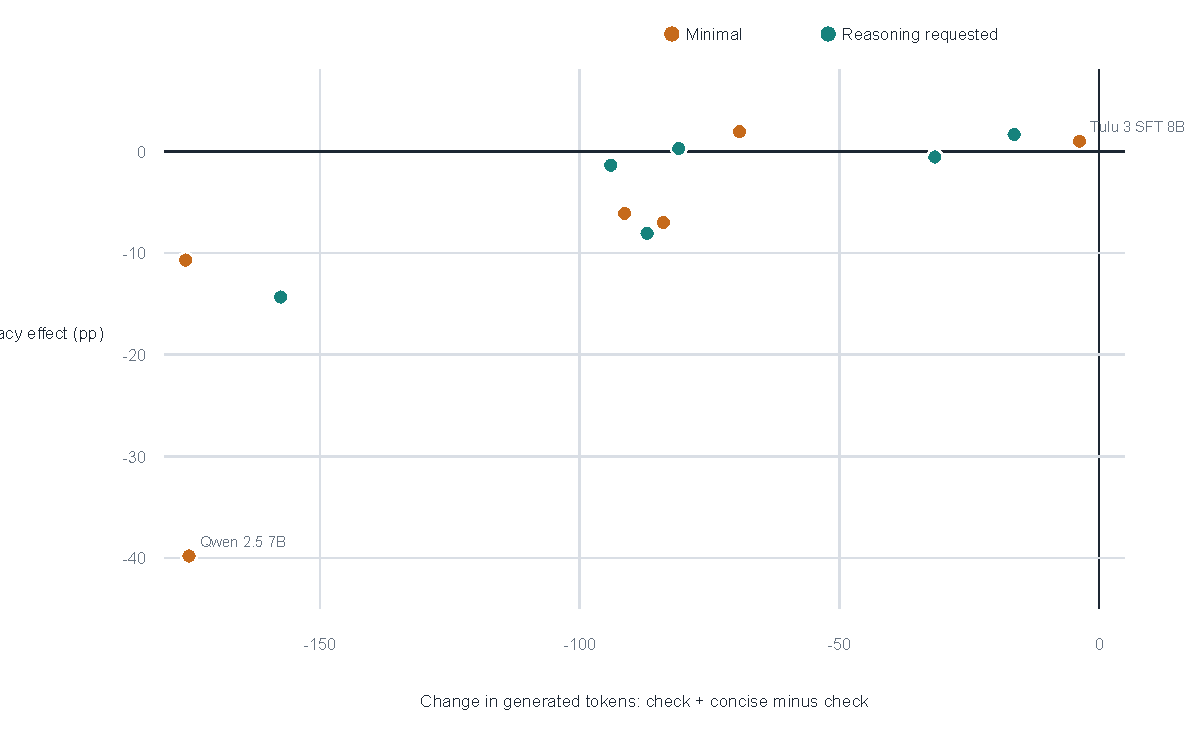
\includegraphics[width=\columnwidth]{figures/results/concision_accuracy_token_tradeoff.pdf}
  \caption{Descriptive accuracy--length tradeoff from adding the concise-output
  constraint to direct checking. Generated-token count is an observable output
  property, not a measure of hidden reasoning.}
  \label{fig:concision-tradeoff}
\end{figure}
